%%%%%%%%%%%%%%%%%%%%%%%%%%%%%%%%%%%%%%%%%
% Simple Sectioned Essay Template
% LaTeX Template
%
% This template has been downloaded from:
% http://www.latextemplates.com
%
% Note:
% The \lipsum[#] commands throughout this template generate dummy text
% to fill the template out. These commands should all be removed when 
% writing essay content.
%
%%%%%%%%%%%%%%%%%%%%%%%%%%%%%%%%%%%%%%%%%

%----------------------------------------------------------------------------------------
%	PACKAGES AND OTHER DOCUMENT CONFIGURATIONS
%----------------------------------------------------------------------------------------

\documentclass[12pt]{article} % Default font size is 12pt, it can be changed here

\usepackage{geometry} % Required to change the page size to A4
\geometry{a4paper} % Set the page size to be A4 as opposed to the default US Letter

\usepackage{graphicx} % Required for including pictures

\usepackage{float} % Allows putting an [H] in \begin{figure} to specify the exact location of the figure
\usepackage{wrapfig} % Allows in-line images such as the example fish picture

\usepackage{csvsimple} % Import CSV Files

\usepackage{lipsum} % Used for inserting dummy 'Lorem ipsum' text into the template
\usepackage{hyperref}

\usepackage{csquotes}
\usepackage[backend=bibtex]{biblatex}

\usepackage[xindy,toc]{glossaries}
\newglossaryentry{computer}
{
  name=computer,
  description={is a programmable machine that receives input,
               stores and manipulates data, and provides
               output in a useful format}
}
\makeglossaries

\bibliography{bib/lit} 

\linespread{1.2} % Line spacing

%\setlength\parindent{0pt} % Uncomment to remove all indentation from paragraphs

\graphicspath{{Pictures/}} % Specifies the directory where pictures are stored

\begin{document}

%----------------------------------------------------------------------------------------
%	TITLE PAGE
%----------------------------------------------------------------------------------------

\begin{titlepage}

\newcommand{\HRule}{\rule{\linewidth}{0.5mm}} % Defines a new command for the horizontal lines, change thickness here

\center % Center everything on the page

\textsc{\LARGE University Name}\\[1.5cm] % Name of your university/college
\textsc{\Large Major Heading}\\[0.5cm] % Major heading such as course name
\textsc{\large Minor Heading}\\[0.5cm] % Minor heading such as course title

\HRule \\[0.4cm]
{ \huge \bfseries Title}\\[0.4cm] % Title of your document
\HRule \\[1.5cm]

\begin{minipage}{0.4\textwidth}
\begin{flushleft} \large
\emph{Author:}\\
John \textsc{Smith} % Your name
\end{flushleft}
\end{minipage}
~
\begin{minipage}{0.4\textwidth}
\begin{flushright} \large
\emph{Supervisor:} \\
Dr. James \textsc{Foo} % Supervisor's Name
\end{flushright}
\end{minipage}\\[4cm]

{\large \today}\\[3cm] % Date, change the \today to a set date if you want to be precise

%\includegraphics{Logo}\\[1cm] % Include a department/university logo - this will require the graphicx package

\vfill % Fill the rest of the page with whitespace

\end{titlepage}



%----------------------------------------------------------------------------------------
%	TABLE OF CONTENTS
%----------------------------------------------------------------------------------------

\tableofcontents % Include a table of contents

\newpage % Begins the essay on a new page instead of on the same page as the table of contents 

%----------------------------------------------------------------------------------------
%	INTRODUCTION
%----------------------------------------------------------------------------------------

\section{Introduction} % Major section

Example citation \cite{Figueredo:2009dg}.

Also there is \cite{bworld}.

Introduction

%------------------------------------------------

\subsection{Subsection 1} % Sub-section

Test here:
A whole lotta text
: and here and \gls{computer}

%------------------------------------------------

\subsubsection{Subsubsection 1} % Sub-sub-section

\lipsum[3] % Dummy text

\begin{figure}[H] % Example image
\center{
\includegraphics[width=0.5\linewidth]{placeholder}}
\caption{Example image.}
\label{fig:speciation}
\end{figure}

%------------------------------------------------

\subsubsection{Subsubsection 2} % Sub-sub-section

description:

\begin{description}
   \item [Name] Foo
   \item [Herkunft] nicht Mitteleuropa
   \item [Vorkommen] Am Rand von Kornfeldern
\end{description}

%----------------------------------------------------------------------------------------
%	HISTORY
%----------------------------------------------------------------------------------------

\section{History} % Major section

History\hfill \\

\csvautotabular{csv/history.csv}
\hfill \\
\hfill \\
test
test
test

%----------------------------------------------------------------------------------------
%	MAJOR SECTION 1
%----------------------------------------------------------------------------------------

\section{Development Methodology} % Major section

\subsection{Process Control}

Process Control

\subsubsection{Definitive Process Control}

lalala\cite{wiki:definedprocess}

\subsubsection{Empirical Process Control}

Wikipedia\cite{wiki:empiricalprocess} lalala.

\subsection{Scrum}
Scrum is a framework for developing and sustaining complex products by Jeff Sutherland and Ken Schwaber. Scrum certification is provided by Scrum Alliance (Chairman Jeff Sutherland \url{https://www.scrumalliance.org/}) and Scrum.org (Founded by Ken Schwaber \url{https://www.scrum.org/}) which together update the official Scrum Guide\cite{scrum:guide}.\newline

Most of what I summarize here can be found directly in the Scrum Guide. Please remember that the Scrum Guide also improves over the years. Those that are still used to Sprint Planning 1 and 2 will find that these meeting no longer exist in that form. Remember, even though Scrum Certification is split between two different companies, they are both working on the same Scrum Guide.\newline

Scrum is free and offered in the Scrum Guide\cite{scrum:guide}. Scrum’s roles, artifacts, events, and rules are immutable and although implementing only parts of Scrum is possible, the result is not Scrum. Scrum exists only in its entirety and functions well as a container for other techniques, methodologies, and practices.

\subsubsection{Overview}

Scrum is founded on empirical process control theory, or empiricism. Empiricism asserts that knowledge comes from experience and making decisions based on what is known. Scrum employs an iterative, incremental approach to optimize predictability and control risk. Three pillars uphold every implementation of empirical process control: transparency, inspection, and adaptation.

Scrum knows \textsc{3 roles}, \textsc{3 artifacts} and \textsc{5 events}.\newline

\fbox{\begin{minipage}{30em}
	Scrum \textbf{does not know} User Stories. Scrum only deals with Product Backlog Items (PBI). It is however common to use User Stories for PBIs.
\end{minipage}}

\subsubsection{3 Roles}
\begin{figure}[H] % Example image
\center{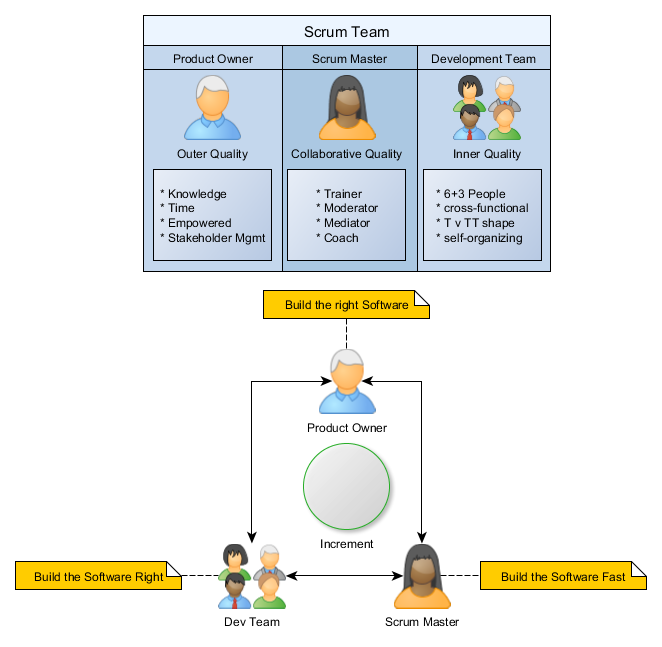
\includegraphics[width=1\linewidth]{Scrum/Roles}}
\caption{Scrum Roles}
\label{fig:scrum:roles}
\end{figure}

\paragraph{Development Team}
\begin{description}
   \item [Name] Dev Team
\end{description}
The Development Team should have a T \cite{wiki:tshaped} or $\pi$ shape. That means that the team should consist of people with a generalist (broad) skill set who are specialists in one (T-shape) specific area. Eventually that team can mature to have generlists who are specialists in two ($\pi$-shape) areas.

\subsubsection{3 Artifacts}

The \textbf{Product Backlog} is an ordered list of everything that might be needed in the product and is the single source of requirements for any changes to be made to the product. The Product Owner is responsible for the Product Backlog, including its content, availability, and ordering. Requirements never stop changing, so a Product Backlog is a living artifact. Multiple Scrum Teams often work together on the same product. One Product Backlog is used to describe the upcoming work on the product.

Product Backlog refinement is the act of adding detail, estimates, and order to items in the Product Backlog. This is an ongoing process in which the Product Owner and the Development Team collaborate on the details of Product Backlog items. Product Backlog items can be updated at any time by the Product Owner or at the Product Owner’s discretion. roduct Backlog items that will occupy the Development Team for the upcoming Sprint are refined so that any one item can reasonably be “Done” within the Sprint time-box. Product Backlog items that can be “Done” by the Development Team within one Sprint are deemed “Ready” for selection in a Sprint Planning.\newline

The \textbf{Sprint Backlog} is the set of Product Backlog items selected for the Sprint, plus a plan for delivering the product Increment and realizing the Sprint Goal. The Sprint Backlog is a forecast by the Development Team about what functionality will be in the next Increment and the work needed to deliver that functionality into a “Done” Increment. Only the Development Team can change its Sprint Backlog during a Sprint. The Sprint Backlog is a highly visible, real-time picture of the work that the Development Team plans to accomplish during the Sprint, and it belongs solely to the Development Team. At any point in time in a Sprint, the total work remaining in the Sprint Backlog can be summed to monitor the progress.\newline

The \textbf{Increment} is the sum of all the Product Backlog items completed during a Sprint and the value of the increments of all previous Sprints. At the end of a Sprint, the new Increment must be “Done,” which means it must be in useable condition and meet the Scrum Team’s definition of “Done.” It must be in useable condition regardless of whether the Product Owner decides to actually release it.

\subsubsection{5 Events, 3 with outputs}

\fbox{\begin{minipage}{35em}
\begin{description}
   \item [Name] Daily Stand-Up
   \item [Duration] Max. 15m
   \item [Participants] Scrum Team (PO optional), open for everyone
   \item [Responsible] Scrum Master
   \item [Input] ?
   \item [Meeting Goal] Shared understanding of where they are
   \item [Questions] \hfill \\ 
    What did I do yesterday that helped the Development Team meet the Sprint Goal?\hfill \\ 
    What will I do today to help the Development Team meet the Sprint Goal?\hfill \\ 
    Do I see any impediment that prevents me or the Development Team from meeting the Sprint Goal?

\end{description}
\end{minipage}}
\newline\newline Only the committed Scrum Team is allowed to talk. Other participants can request talking rights from the Scrum Master. The Daily is almost self moderating. The \textbf{Rule of two Hands} allows two or more independent people to raise their hands when a topic for them is unimportant. Then the topic is dropped immediately. You can also ask the team if they believe that they can fulfill the sprint goal. The Scrum Team Members vote with their thumbs (Up, middle, down) which leads to more discussions. You can also update the Sprint Burndown Chart.\newline

\fbox{\begin{minipage}{35em}
\begin{description}
   \item [Name] Sprint Planning
   \item [Duration] Max. 8h
   \item [Participants] Scrum Team, Stakeholder
   \item [Responsible] Scrum Master
   \item [Input] Ordered, sufficiently filled Backlog\hfill \\ 
		A Sprint Goal by the PO (or the Dev Team)
   \item [Meeting Goal] Shared understanding of what to do and how
   \item [Output] Sprint Backlog (Commitment of the Scrum Team)
\end{description}
\end{minipage}}
\newline\newline Text about the Sprint Planning\newline

\fbox{\begin{minipage}{35em}
\begin{description}
   \item [Name] Sprint Review
   \item [Duration] Max. 4h (30m to 1h is sensible)
   \item [Participants] Scrum Team, Key Stakeholders (invited by PO)
   \item [Responsible] Scrum Master
   \item [Input] Potentially Shippable Product (in neutral customer environment)\hfill \\ 
		Product Owner ensures Product Backlog and Roadmap are presentable.
   \item [Meeting Goal] Know where we are and how to continue.
   \item [Output] Feedback, Customer Happiness, Revised Product Backlog that defines the probable Product Backlog items for the next Sprint
	 \item [Note] During the Review the PO can actively manage the present Stakeholders. Stories are no longer accepted/rejected during the Sprint Review (since 2013). Accepting/Rejecting Stories is the job of the Product Owner and happens during the Sprint, whenever a story is ready.
\end{description}
\end{minipage}}
\newline\newline Text about the Sprint Review\newline


\fbox{\begin{minipage}{35em}
\begin{description}
   \item [Name] Sprint Retrospective
   \item [Duration] Max. 3h (2h is sensible)
   \item [Participants] Scrum Team \textbf{Only}
   \item [Responsible] Scrum Master
   \item [Input] Pro/Contra for each Scrum Team Member. Scrum Master prepares Topics.
   \item [Meeting Goal] Know where we are and how to continue.
   \item [Output] Action Items (tackle 2/3 items in the next sprint)(sensible things should not be on the sprint board)
\end{description}
\end{minipage}}
\newline\newline This meeting is team and process focused. Other meetings are focused on the product.\newline

\subsubsection{Defintion of \ldots}

Definiton of Ready:
\begin{itemize}
		\item Story has Business Value
    \item Story has been reviewed and estimated by the team
    \item Story is complete in format - User X needs to Y so they can Z
    \item Acceptance criteria are clear and agreed upon
		\item dependencies identified and ready or mitigation agreed
		\item Product Owner has approved the story
\end{itemize}

Definiton of Done:
\begin{itemize}
    \item Acceptance tests written and pass (Meets acceptance criteria)
    \item Unit and Integration tests written and pass
    \item Code peer reviewed and approved
		\item Code is meeting development standards (e.g. as defined in Checkstyle)
    \item Code committed to repository
		\item Deployed to system test environment and passes system tests
		\item Any build/deployment/configuration changes implemented/documented/communicated
    \item QA testing done (by team members other than those working on the implementation of that feature)
		\item Smoke tests performed on dev/staging environment
    \item Product Owner signed off
\end{itemize}

Release Definiton of Done:
\begin{itemize}
    \item Acceptance, Unit and Integration tests pass
    \item Configuration changes are ready
		\item Tag created for the release
\end{itemize}

Bug Definiton of Done:
\begin{itemize}
    \item The Defect is fixed
    \item if missing, Unit Tests are implemented that covers the fix’s code functionality
		\item a functional test to cover the bug is performed by a person other than the person who fixed the bug
		\item an automated test is created that checks the flow
\end{itemize}

\subsection{Kanban}

%----------------------------------------------------------------------------------------
%	MAJOR SECTION 1
%----------------------------------------------------------------------------------------

\section{Patterns} % 

Patterns

\subsection{CQRS}



%------------------------------------------------
\section{Three}
\subsection{Subsection 1} % Sub-section

\subsubsection{Subsubsection 1} % Sub-sub-section

\lipsum[6] % Dummy text

%------------------------------------------------

\subsubsection{Subsubsection 2} % Sub-sub-section

\lipsum[6] % Dummy text
\begin{wrapfigure}{l}{0.4\textwidth} % Inline image example
  \begin{center}
    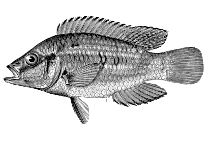
\includegraphics[width=0.38\textwidth]{fish}
  \end{center}
  \caption{Fish}
\end{wrapfigure}
\lipsum[7-8] % Dummy text

%------------------------------------------------

\subsubsection{Subsubsection 3} % Sub-sub-section

\begin{description} % Numbered list example

\item[First] \hfill \\
\lipsum[9] % Dummy text

\item[Second] \hfill \\
\lipsum[10] % Dummy text

\item[Third] \hfill \\
\lipsum[11] % Dummy text

\end{description} 

%----------------------------------------------------------------------------------------
%	MAJOR SECTION X - TEMPLATE - UNCOMMENT AND FILL IN
%----------------------------------------------------------------------------------------

%\section{Content Section}

%\subsection{Subsection 1} % Sub-section

% Content

%------------------------------------------------

%\subsection{Subsection 2} % Sub-section

% Content

%----------------------------------------------------------------------------------------
%	CONCLUSION
%----------------------------------------------------------------------------------------

\section{Conclusion} % Major section

\lipsum[12-13]

%----------------------------------------------------------------------------------------
%	BIBLIOGRAPHY
%----------------------------------------------------------------------------------------
\printbibliography 

%----------------------------------------------------------------------------------------
%	GLOSSARY
%----------------------------------------------------------------------------------------
\printglossaries

%----------------------------------------------------------------------------------------
\end{document}